\chapter[Modeling Plagiarism Detection]{Token-based Plagiarism Detection for Artifacts of Modeling Assignments}\label{sec:mde-approach}

\noindent
In this chapter, we address the problem of modeling plagiarism detection (\probref{2}) by introducing a novel approach to enable token-based plagiarism detection for modeling assignments (\contribution{2}). 
Where applicable, we reuse concepts of token-based approaches that are compatible with modeling artifacts, adapting only those components that are inherently incompatible with the unique characteristics of modeling languages.
With this, we provide resilience against obfuscation techniques and allow state-of-the-art token-based plagiarism detection systems to extend their scope beyond code-based approaches.
%
With this approach, we address the challenges discussed in \autoref{sec:mde-challenges}.

For our approach, modeling artifacts that are EMOF-conforming~\cite{MOF2016a} or that have an underlying tree-like structure are particularly suited, but our approach can be generalized beyond them. Supported modeling artifacts include (domain) models, metamodels, but also model transformations and model queries, as they can be represented as models themselves~\cite{Bezevin2005, Martinez2020},

The remainder of the chapter is structured as follows.
First, we discuss the difficulty of defining intrusiveness for modeling artifacts.
Second, we provide a minimal running example for the remainder of this chapter.
Next, we provide an overview of our approach. We explore the primary challenge of tokenizing modeling artifacts and examine the required normalization steps. We address the pairwise matching of subsequences, detail the similarity calculation, and the result visualization. Finally, we conclude with a discussion of the limitations.

\ownpublications{
    \fancycite{Saglam2024a},
    \fancycite{Saglam2023},
    \fancycite{Saglam2022}, and
    \fancycite{Kienzle2024}.
}

\section{Intrusiveness in Model Obfuscation}\label{sec:mde-intrusiveness}
As discussed in \autoref{sec:mde-challenges}, the differentiation between semantic-preserving, semantic-agnostic, and semantic-deviating obfuscation is blurred in the context of modeling plagiarism, as for metamodels dynamic semantics are often only informally specified~\cite{Brambilla2017}.
To address this issue, we thus distinguish two cases: 


If there is there are formally described dynamic semantics for a given metamodel, we can define the \textit{intrusiveness} (see \autoref{sec:intrusiveness}) analogous to \autoref{def:spoa}, \autoref{def:saoa} and \autoref{def:sdoa}, but instead of the functional equivalence as defined in \autoref{def:func-eq} we use the semantic equivalence of models:
\begin{theorem}[Semantical Equivalence of Models]\label{def:sem-eq}
Let \(M_1, M_2 \in \mathcal{M}\) be models of a metamodel \(\mathcal{M}\). 
We denote the semantic equivalence of two models \(M_1\) and \(M_2\) by the binary relation \(\equiv_{\mathcal{M}} \, \subseteq \mathcal{M} \times \mathcal{M}\).
% where \(M_1 \equiv_{\mathcal{M}} M_2\) iff \(M_1\) and \(M_2\) are semantically equivalent.
\end{theorem}

If there are no formally described dynamic semantics for a given metamodel, but we can define a transformation between the metamodel and a formalism with well-defined semantics, we can define derived semantic equivalence as follows.
\begin{theorem}[Derived Semantical Equivalence of Models]\label{def:sem-eq-derived}
Let \(M_1, M_2 \in \mathcal{M}\) be models of the metamodel \(\mathcal{M}\). Furthermore, let \(\mathcal{P}\) be a formalism with well-defined semantics and let \(P_1, P_2 \in \mathcal{P}\) be representations of \(\mathcal{P}\) for which semantical equivalence is denoted by the binary relation \(\equiv_\mathcal{P} \, \subseteq \mathcal{P} \times \mathcal{P}\).
Suppose there exists a transformation \(t: \mathcal{M} \rightarrow \mathcal{P}\) such that
\[
M_1 \xrightarrow{t} P_1 \quad \text{and} \quad M_2 \xrightarrow{t} P_2 \,.
\]
Then, we define the derived semantic equivalence on \(\mathcal{M}\) as follows:
\[
P_1 \equiv_{\mathcal{P}} P_2 \quad \implies \quad M_1 \equiv_{\mathcal{M}} M_2.
\]
\end{theorem}

As for program code, the distinction regarding intrusiveness in the context of models is useful, as it allows categorizing and reasoning about different types of obfuscation attacks. However, a difference between any two models, for example, derived via model differencing, that reflects a semantic-preserving change is not evidence for obfuscation. It is actually impossible to categorically decide which types of differences between the two models constitute obfuscation and are thus formal evidence for plagiarism, even under a clear definition of intrusiveness. Plagiarism detection must \textit{always} involve human inspection at the end, where this decision is made on a case-by-case basis (see \autoref{sec:foundations-pds}).

\section{Running Example}
\label{sec:mde-example}

\begin{figure}[b]
    \centering
    \begin{subfigure}{.96\textwidth}
        \centering\captionsetup{width=.95\linewidth}%
        \caption{First example metamodel.}
        \label{fig:sub1}
        %\includegraphics[width=.89\textwidth]{images/bookStore2.pdf}
        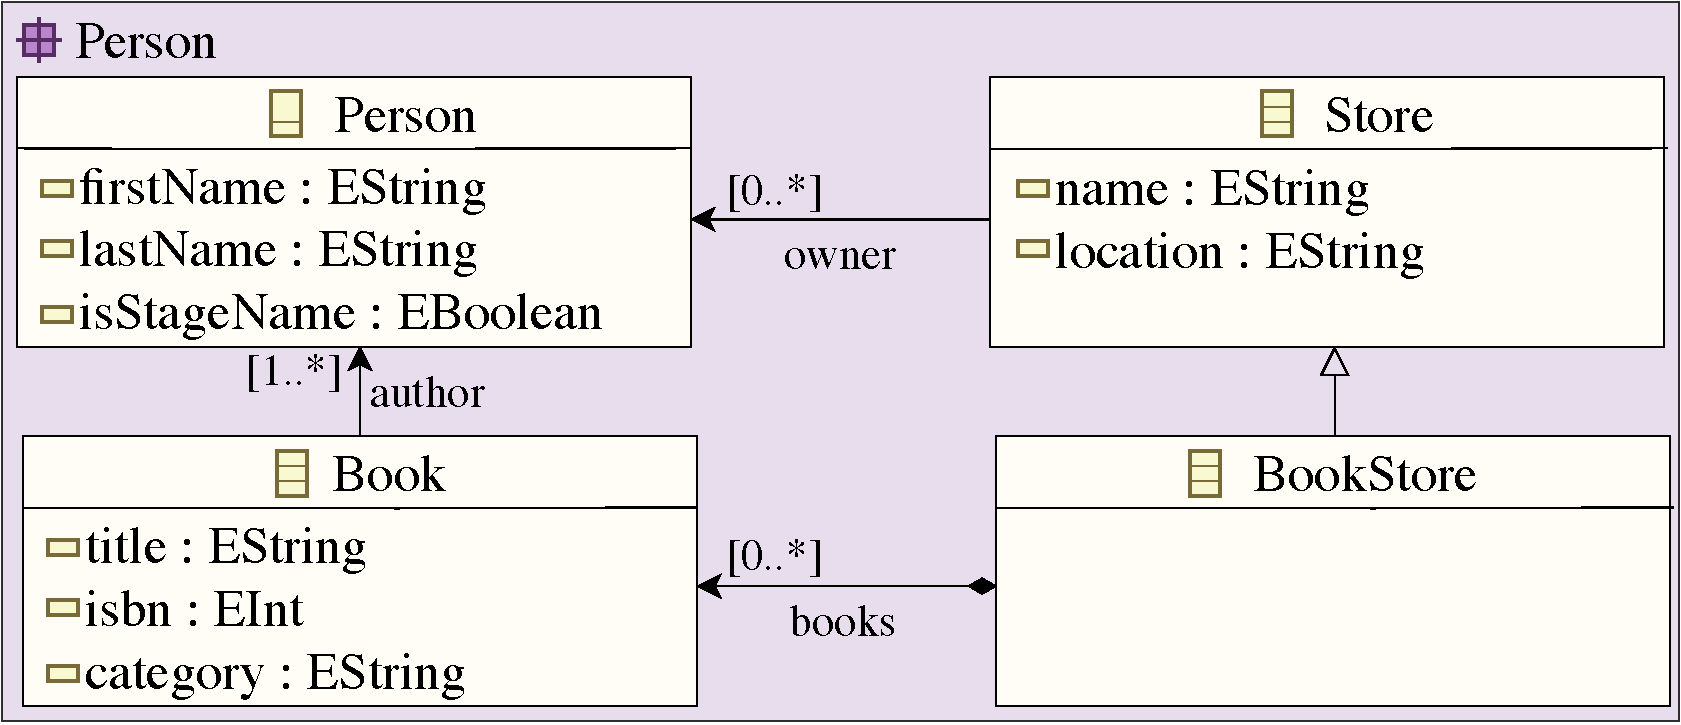
\includegraphics[width=.8\textwidth]{figures/mde/bookstore-1.drawio.pdf}
    \end{subfigure}  
    
    % This comment needs to stay, or the figures will not be side-by-side. Yes, this is not a joke. 
    \begin{subfigure}{.96\textwidth}
          \centering\captionsetup{width=.95\linewidth}%
        \caption{Second example metamodel.}
          \label{fig:sub2}
          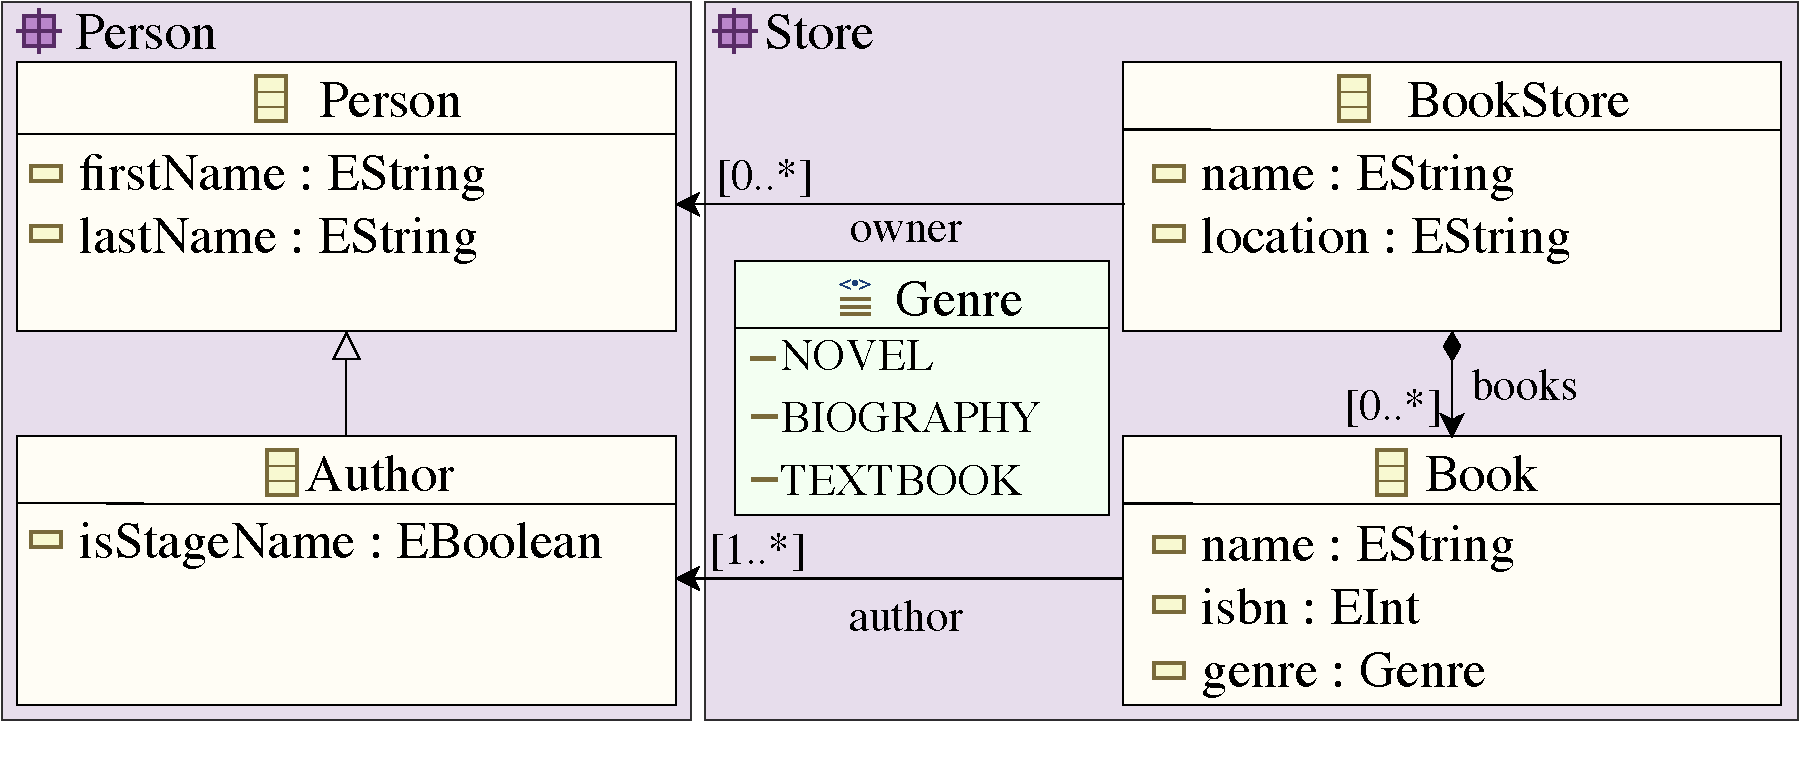
\includegraphics[width=.8\textwidth]{figures/mde/bookstore-2.drawio.pdf}
    \end{subfigure}
    \caption[Running Example: Bookstore Models]{Two similar but not identical example models representing a bookstore management system that allows managing multiple stores and their inventory.}
    \label{fig:running-example}
%\end{figure*}
\end{figure}
%
% SETUP
\noindent
As a minimal running example, we consider an undergraduate course where students are instructed in the elementary principles of modeling. Such a course is typical according to the survey of \citet{Ciccozzi2018}.
In order to satisfy the course requirements, they need to complete an assignment that entails modeling a management system for bookstores, requiring the creation of an appropriate metamodel.
% DOMAIN
The domain is described as follows:
\begin{myquote}
\small
\textit{Bookstore can have multiple locations that sell different books.
Books are classified into different genres and have a unique identifier called an ISBN.
Books have an author who may use a stage name. Stores have one owner.  }
\end{myquote}
This example is intentionally small to illustrate our approach and provide clarity for the reader; most modeling assignments are usually more comprehensive.
Two potential solutions for this assignment are depicted in \autoref{fig:running-example}.
% PROBLEM
Although they exhibit some similarities, several features are modeled differently.
While this is a small task, it is hard for a human to determine how similar these models are even for these two solutions.
However, in a course, there may be 30 to 300 students~\cite{Ciccozzi2018}. Thus, manual checking for plagiarism becomes impractical.
%\todo{expand? What is different? What are the similarities? Obviously, as a running example, it is too small to label something plagiarism, but it is still very complex to assess similarity.}

\section{Overview}\label{sec:mde-approach-overview}
The similarity between models and code can be leveraged for token-based approaches for modeling artifacts \cite{Saglam2022}.
These approaches typically extract tokens from parse tree nodes, primarily focusing on the code's structure.
In contrast, for modeling plagiarism, the focus must be on modeling patterns, structure, and relationships.
A key challenge is the higher abstraction than code, where the lack of details impedes plagiarism detection.
Furthermore, resilience against re-ordering-based obfuscation attacks is challenging.
Re-ordering-based attacks are more common \cite{Saglam2023} as they are considerably more accessible for most models than for code, where the sequence of statements determines the code's behavior.
% MODEL vs. CODE END
In our approach, modeling assignment solutions undergo a comprehensive pairwise comparison process.
To facilitate this comparison, an abstraction layer is extracted from each solution, on which the structures of these artifacts are compared.
Ultimately, our approach produces a list of suspicious solutions, which are the subject of the instructor's final evaluation.
% HUMAN FACTOR
As with all plagiarism detection systems, the human component of the process is critical for ethical reasons, as it can ultimately only be up to the instructor to decide whether a submission constitutes plagiarism~\cite{Culwin2001, Weber2019}.
Our approach combines the strengths of automated analysis with human judgment, offering an ethical approach to detecting plagiarism in modeling assignments.
%
% APPROACH OVERVIEW
As other token-based approaches~\cite{prechelt2002, Maertens2022}, our approach consists of five steps.
\begin{enumerate}%[leftmargin=*]
    \item \textbf{Tokenization}: We generate the token sequence by linearizing the model, extracting tokens for particular model elements, and abstracting from superfluous detail.
    \item \textbf{Normalization}: We achieve resilience against element reordering by normalizing the token sequence. This can be combined with other normalization techniques.
    \item \textbf{Pairwise Matching}: We efficiently compare pairs of token sequences to find the longest matching subsequences greedily, thus matching fragments of modeling artifacts.
    \item \textbf{Similarity Calculation}: We rank the pairs by leveraging different similarity metrics for the matches of a pair. Post-processing steps, such as clustering analysis, can be applied.
    \item \textbf{Visualization}: We visualize matching fragments between modeling artifacts via textual syntaxes to help educators assess the results and decide what constitutes plagiarism effectively.
\end{enumerate}
The novelty of our approach lies in steps 1, 2, and 5, while steps 3 and 4 are established techniques from token-based plagiarism detection.

% ------------------------------------------------------------------
% 1. TOKENIZATION
% ------------------------------------------------------------------

\section{Tokenization}\label{subsec:tokenization}


\noindent
Modeling assignments include diverse artifacts like metamodels, models, and other artifacts~\cite{Ciccozzi2018}, all vital in the modeling process.
Most of these artifacts are typically systematized in a tree-like structure. Throughout this section, we will mainly refer to models and their elements. However, our approach applies to other tree-based modeling artifacts, such as metamodels, et cetera.
%
Our approach transforms the modeling artifacts into an abstraction layer on which pairwise comparison can be performed. By omitting \textit{some} details while including others, mainly structural information, this abstraction layer is resilient against certain obfuscation attacks such as renaming and re-typing.
For example, we omit the names of elements and the exact types of attributes, as they are usually the first to be changed for obfuscation purposes~\cite{Saglam2022, Saglam2023}.
%
To tokenize models of a given modeling language, one first has to identify the primary \textit{tokenization references} in the modeling language.
%
\begin{concept}[Tokenization References]\label{def:semantic-ref}
    In the context of modeling plagiarism detection, the explicit references or connections within a model define its semantic aspects, dictating the meaning and behavior of the model elements. They are domain-specific relationships between elements within a model that influence the interpretation or execution behavior of the model. They are crucial for tokenization and thus have to be identified for each modeling language or domain. We call them tokenization references.
\end{concept}
%
These references are crucial in both structural and behavioral models. In structural models, tokenization references typically take the form of containment relationships, defining the hierarchical organization of elements. 
Tokenization references can take various forms in behavioral models, including dynamic references such as state transition references in state charts. Tokenization references are used to determine the order in which to tokenize the model elements.

\begin{theorem}[Tokenization]\label{def:tokenization}
Let \(M \in \mathcal{M}\) be a model which is an instance of Metamodel \(\mathcal{M}\) with elements \(\mathcal{E}_M\), and let \(\mathcal{C}_\mathcal{M}\) denote the set of metaclasses in the metamodel.
We define a left total relation, where \( \mathcal{T}_\mathcal{M} \in \mathbb{N} \cup \{\bot\} \) is the set of possible tokens for \(\mathcal{M}\),
\begin{align*}
    \operatorname{tokenize}_\mathcal{M}: \mathcal{E}_M \rightarrow \mathcal{T}_\mathcal{M}
\end{align*}
that assigns either a token \( t \in \mathcal{T}_\mathcal{M} \) or no token \( \bot \) to each element \( e \in \mathcal{E}_M \).
\end{theorem}

In our approach, we tokenize as follows:
\begin{enumerate}
    \item We iterate in a depth-first order over the tree structure of the model's tokenization references, starting from its root element.
    \item For each element, we decide what tokens may be extracted. The extraction strategy can either be generic or domain-specific.
    \item Token sequences from multiple files or artifacts are concatenated into one token sequence but separated via a pivot token.
\end{enumerate}

\autoref{alg:model-tokenization} shows such an algorithm for tokenizing models, which incorporates the three aforementioned steps.
Here, the function \textsc{Tokenize} is a mapping that provides a token for any given model element or no token (\(\bot\)) if none shall be extracted for a given element (see \autoref{def:tokenization}).
In the case of multiple root elements, the token sequence of the corresponding root elements can be concatenated.

\begin{algorithm}[H]
\caption{Recursive Tokenization of a Model}
\label{alg:model-tokenization}
\begin{algorithmic}[1]
\Require Model $M$ with root element $r$
\Ensure Token sequence \((t_i)_{i=1}^{l}\) representing the model $M$
\State Initialize empty token sequence: $(t_i) \gets (\,)$
\Function{TokenizeModel}{$r, (t_i)$}
    \State $(t_i) \gets (t_i) \, \cdot$ \textsc{Tokenize}$(r)$

    \For{each Element $e$ reference via tokenization references of $r$}
        \State $(t_i) \gets (t_i) \, \cdot$ \textsc{TokenizeModel}$(e, (t_i))$
    \EndFor
    \State \Return $(t_i)$
\EndFunction
\end{algorithmic}
\end{algorithm}

\noindent
As an example, \autoref{fig:tokenization} illustrates the tokenization for the domain of \ac{EMF} metamodels using our running example. In the case of \ac{EMF} metamodels, the tokenization references are the \textit{containment references}. The metamodel is depicted in a typical tree view, where the indentation signifies the containment relations.
The token tree (\autoref{fig:tokenization:sub1}) is linearized into a token sequence according to \autoref{alg:model-tokenization} (\autoref{fig:tokenization:sub2}). Each token represents information from the structure of the metamodel and is thus an abstract representation of the metamodel.

%We discuss two kinds of strategies for selecting tokens: 
There are generally two possible types of strategies for mapping modeling elements to tokens (which is the role \textsc{Tokenize} fulfills in \autoref{alg:model-tokenization}): \textit{generic strategies} and \textit{domain-specific strategies}.
%
The first kind is \textit{generic strategies}, where a token is extracted for each model element, and the identity of the token is the type of the element, the metaclass, respectively.

\begin{theorem}[Metaclass Instantiation]
Let \(M \in \mathcal{M}\) be a model which is an instance of Metamodel \(\mathcal{M}\) with elements \(\mathcal{E}_M\), and let \(\mathcal{C}_\mathcal{M}\) denote the set of metaclasses in the metamodel. For each element \( e \in \mathcal{E}_M \), there exists a unique metaclass \( C \in \mathcal{C}_\mathcal{M} \) such that \(e\) is an instance of \( C \). We denote this right-unique relationship with the operator
\begin{align*}
:: \, \subseteq \mathcal{E}_M \times \mathcal{C}_\mathcal{M} \,.
\end{align*}
\end{theorem}

\begin{theorem}[Generic Tokenization Strategy]\label{def:generic-strat}
Let \(M \in \mathcal{M}\) be a model which is an instance of Metamodel \(\mathcal{M}\) with elements \(\mathcal{E}_M\), and let \(\mathcal{C}_\mathcal{M}\) denote the set of metaclasses in the metamodel.

We define a surjection \( \operatorname{tokenize}_{generic}: \mathcal{E}_M \rightarrow \mathcal{T}_\mathcal{M} \), where \( \mathcal{T}_\mathcal{M} \) is the set of possible tokens for \(\mathcal{M}\), that assigns a token \(t_C \in \mathcal{T}_\mathcal{M}\) based on metaclass \( C \in \mathcal{C}_\mathcal{M} \) to each element \( e \in \mathcal{E}_M\) such that
\begin{align*}
    \forall e \in \mathcal{E}_M, \; \exists_1 t_C \in \mathcal{T}_\mathcal{M} \quad : \quad 
    \operatorname{tokenize}_{\text{generic}}(e) = t_C \iff e :: C \,.
\end{align*}
\end{theorem}
However, the generic strategy as defined in \autoref{def:generic-strat} has certain limitations. Some model elements are irrelevant and should not be extracted as tokens, as they increase the noise in the token sequence and can be used to obfuscate plagiarism. Additionally, the properties of elements are not represented in the token sequence at all. If these properties are semantically relevant, this leads to a lack of representation in the token sequence. When considering \ac{EMF} metamodels as an example, classes and interfaces are differentiated by a property.
While this generic strategy can be applied to any modeling language and thus to any modeling assignment artifacts, it may perform worse for a distinct domain than a strategy specifically tailored to one domain. However, a generic strategy may perform well enough for some modeling languages (mostly those where the essential information is provided by the model elements instead of their properties and relations). 

The second kind type of strategy is \textit{domain-specific strategies}, where the selection of tokens is designed for a single domain or modeling language.
This allows more fine-grained rules for mapping model elements to tokens. Thus, \autoref{def:generic-strat} no longer applies, as there is not necessarily a bijective mapping between metaclasses and token types. In the following, we discuss several possible rules that allow deviating from a generic tokenization strategy.

\begin{theorem}[Token Omission]\label{def:token-omission}
Let \( \operatorname{tokenize}_\mathcal{M}: \mathcal{E}_M \rightarrow \mathcal{T}_\mathcal{M} \) be a tokenization function according to \autoref{def:tokenization}. 
We refer to \( \operatorname{tokenize}_\mathcal{M}\) as a tokenization function with token omission if there is a model element\( e \in \mathcal{E}_M \) which does not map to any token, and thus the following applies:
\begin{align*}
       \operatorname{tokenize}_\mathcal{M}(e) = \bot \,.
\end{align*}
\end{theorem}

Model elements that can be omitted without changing the semantics of a model should not tokenized, as these elements can be exploited to affect the token sequence via an obfuscation attack. To that end, a token omission rule can be employed. This can be useful, for example, for typed elements, where the type should not be extracted as a token.
\autoref{fig:tokenization} illustrates an exemplary domain-specific tokenization for \ac{EMF} metamodels. As seen in \autoref{fig:tokenization:sub2}, we extract tokens for attributes, but no tokens are extracted for the values of these attributes.

\begin{theorem}[Token Collision]\label{def:token-collision}
Let \( \operatorname{tokenize}_\mathcal{M}: \mathcal{E}_M \rightarrow \mathcal{T}_\mathcal{M} \) be a tokenization function according to \autoref{def:tokenization}. 
We refer to \( \operatorname{tokenize}_\mathcal{M}\) as a tokenization function with token collision if there is a pair of distinct elements \( e_1, e_2 \in \mathcal{E}_M \), where \( e_1 \) and \( e_2 \) belong to different metaclasses \(C_1, C_2 \in \mathcal{C}_\mathcal{M}\) with \( e_1 :: C_1, \, e_2 :: C_2, \, C_1 \neq C_2 \) but produce the same token \(t \in \mathcal{T}_\mathcal{M}\) and thus the following applies:
\begin{align*}
       \operatorname{tokenize}_\mathcal{M}(e_1) = \operatorname{tokenize}_\mathcal{M}(e_2) \, .
\end{align*}
\end{theorem}

Two elements of a different type that can be used interchangeably without changing the semantics of the modeling artifact should map to a token with the same identity. To that end, a token collision rule can be employed.
Consider a metamodel for component-based software modeling as an example. If there are different ways of modeling a component, for example, via classes or via packages, but for the sake of the modeled architecture, they can be used interchangeably, then they should map to the same token representing components.

\begin{theorem}[Token Distinction]\label{def:token-distinction}
Let \( \operatorname{tokenize}_\mathcal{M}: \mathcal{E}_M \rightarrow \mathcal{T}_\mathcal{M} \) be a tokenization function according to \autoref{def:tokenization}. We refer to \( \operatorname{tokenize}_\mathcal{M}\) as a tokenization function with token distinction if there is a pair of distinct elements \( e_1, e_2 \in \mathcal{E}_M \), where \( e_1 \) and \( e_2 \) belong to the same metaclasses \(C \in \mathcal{C}_\mathcal{M}\) with \( e_1 :: C, \, e_2 :: C\) but produce different tokens \(t_1, t_2 \in \mathcal{T}_\mathcal{M}\) based on, for example, their values for a property of \(C\). Thus, the following applies:
\begin{align*}
       \operatorname{tokenize}_\mathcal{M}(e_1) \neq \operatorname{tokenize}_\mathcal{M}(e_2) \, .
\end{align*}
\end{theorem}

In contrast, elements of the same type that, through their properties, have different semantics should be mapped to different tokens.
To that end, a token distinction rule can be employed.
Note that a tokenization function can have token distinction, token collision, and token omission, as it consists of a set of mapping rules from model elements to tokens.
As seen in \autoref{fig:tokenization:sub2}, attributes and identifier attributes are extracted as different tokens, even though both are instances of the same metaclass. Here, the property of the attribute defines whether it is an identifier or not.
Similarly, this is done for references and containment references.
Finally, properties themselves may lead to the extraction of tokens, for example, for supertype references or similar (see \autoref{fig:tokenization:sub2}).

In summary, tokenization requires finding a suitable mapping between the set of model elements of a modeling language and a set of tokens, as defined by \autoref{def:tokenization}, to maximize the detection quality and obfuscation resilience. This has to be done for each modeling language or domain, as there is no universal mapping for all languages that fulfill this task. Ideally, finding such a mapping involves a domain expert in order to consider the particularities and ambiguities of that domain.
%
Selecting how model elements map to tokens for tokenization in token-based plagiarism detection requires careful consideration of the relevant elements and properties of the domain. A domain-specific strategy allows for a more fine-grained tokenization and is thus generally preferred. A generic strategy, however, remains a baseline for domains without a domain-specific strategy.

\begin{figure}
    \centering
    \begin{subfigure}{.45\linewidth}
        \centering\captionsetup{width=.99\linewidth}%
        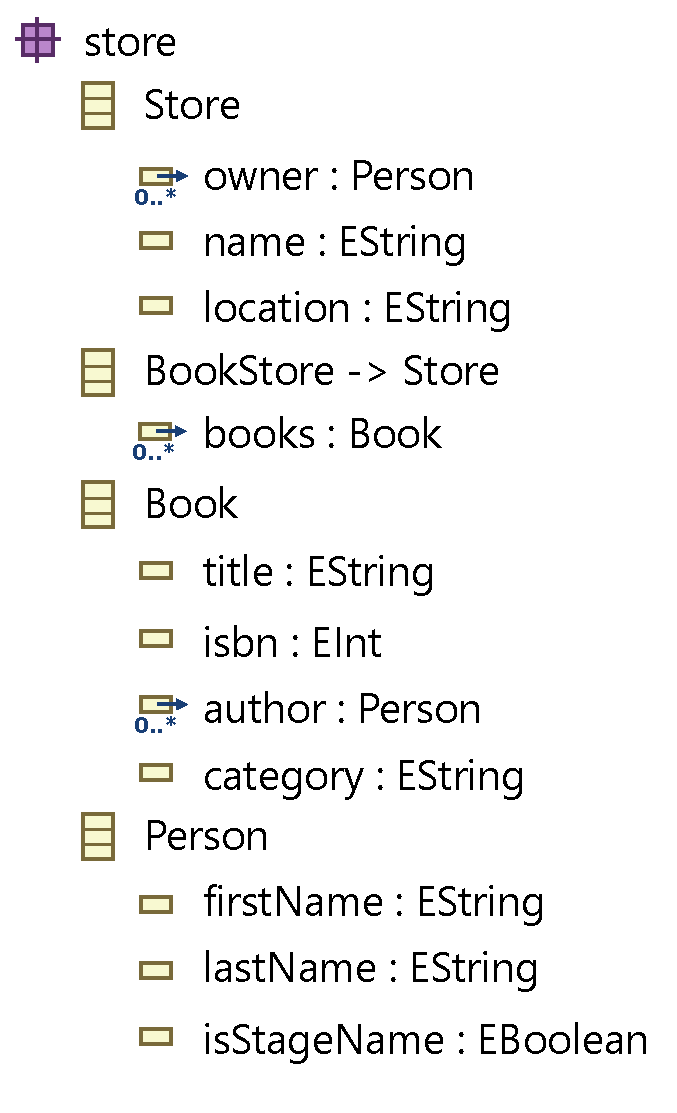
\includegraphics[width=.90\textwidth]{figures/mde/emfTreeView.pdf}
        \caption{first example metamodel}
        \label{fig:tokenization:sub1}
    \end{subfigure}% This comment needs to stay, or else the figures will not be side-by-side. Yes, this is not a joke.
    \begin{subfigure}{.45\linewidth}
          \centering\captionsetup{width=.99\linewidth}%
          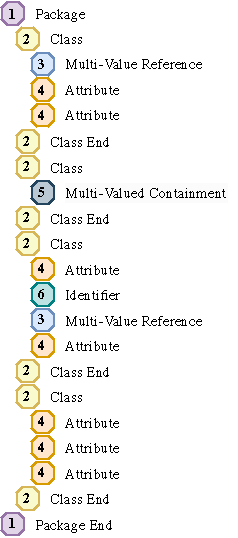
\includegraphics[width=.65\textwidth]{figures/mde/tokenSequence.pdf}
          \caption{extracted token sequence}
          \label{fig:tokenization:sub2}
    \end{subfigure}
    \caption[Tokenization of Modeling Artifacts]{Tokenization of one of the example models in \autoref{fig:running-example} to extract a linear token sequence as an abstraction layer for the comparison.}
    \label{fig:tokenization}
\end{figure}

\subsection{Tokenizing EMF Metamodels}
To continue our running example, we now discuss how to tokenize \ac{EMF} metamodels. This enables, for example, plagiarism detection for modeling assignments such as the one described in \autoref{sec:human-plagiarism-task}. However, these tokenization rules can be adapted for similar structural models with little effort. For example, the rules can be directly transferred to \ac{UML} class models, as \ac{EMF} is EMOF-compliant. As previously mentioned, in the case of \ac{EMF} metamodels, the tokenization references are the containment references. We discuss both a generic and a domain-specific strategy.

\subsubsection{Generic Strategy}
For the generic Strategy, we define the set of possible tokens based on the concrete metaclasses of the meta-metamodel as described in \autoref{def:generic-strat}.
To extract the tokens, we traverse the metamodel and extract tokens containing only the metaclass of the element as information. Properties like the element name are not transferred. This approach thus extracts tokens for packages, classifiers, attributes, references, etcetera.
\autoref{fig:ecore-tokenization} visualizes the inheritance tree of the Ecore meta-metamodel. The information extracted by the generic token selection is shown in blue and green. As the Ecore meta-metamodel is self-describing and self-instantiating, the generic token selection can be applied to their instances in addition to metamodels.
%
However, the generic token selection comes with two downsides.
As a first problem, it also extracts tokens with very little meaning. We observed \texttt{EGenericType} to be especially problematic, as \ac{EMF} automatically creates an \texttt{EGenericType} for every \texttt{ETypedElement} in a metamodel.
As a second problem, some vital information is not transferred into tokens. \ac{EMF} distinguishes concrete classes, abstract classes, and interfaces via two flags stored as attributes in the metaclass \texttt{EClass}.
Thus, the generic token selection only extracts class tokens and cannot make a more precise distinction. Analogously, containment references are not distinguished from regular references, and identifier attributes are not distinguished from regular attributes.

\subsubsection{Domain-Specific Strategy}
The domain-specific token strategy builds upon the previous strategy. It also uses metaclasses to extract tokens. However, it employs several tokenization rules for several types of model elements.
Compared to the generic strategy, there are three key differences in the token set:
\begin{enumerate}
    \item \textit{Stricter Token Selection}. The concrete metaclasses \texttt{EFactory}, \texttt{EGenericType}, and \texttt{EObject} are not extracted as tokens. They provide superfluous information as they are rarely explicitly modeled by a student. Thus, they needlessly increase the attack surface by allowing changes to the token sequence that do not alter the semantics of the metamodel (these are token omission rules as defined in \autoref{def:token-omission}).
    \item \textit{Token Distinction via Attributes}. Some concrete metaclasses are further distinguished to extract more fine-grained information. An \texttt{EClass} can be a class, abstract class, or interface. Containment references have a different token type compared to non-containment ones. Analogously, identifier attributes differ from normal attributes. This distinction broadens the token set and thus reduces false positives, as the discerned model elements semantically serve very different purposes (these are token distinction rules as defined in \autoref{def:token-distinction}).
    \item \textit{Extraction from Meta-References}. Some tokens are extracted for important meta-references in the Ecore meta-metamodel. Each superclass reference of an \texttt{EClass} is extracted as \textit{super type} token, and a return type reference of each non-void \texttt{EOperation} is extracted as \textit{return type} token (this is not possible via a generic strategy, as these references are not classes).
Again, these additional tokens reduce false positives. Moreover, they allow the detection of additional similarities, like the number of declared supertypes.
\end{enumerate}
%
As depicted in \autoref{fig:ecore-tokenization}, fewer concrete metaclasses are used for tokens. However, additional information is used to distinguish more token types.
In contrast to the generic token selection, this domain-specific strategy is tailored explicitly towards metamodels and thus not applicable to their instances. However, while it tends to extract fewer tokens than the generic strategy for the same input, it can differentiate between more token types through its refined and extended token set.


\begin{figure}
    \centering
    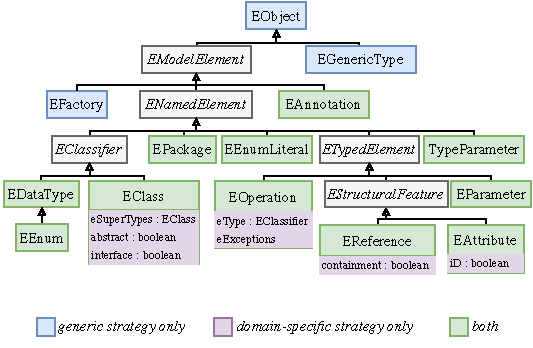
\includegraphics[width=0.85\linewidth]{figures/mde/Ecore-Both.pdf}
    \caption[EMF Metamodel Tokenization Strategies]{Tokenization rules for \ac{EMF} metamodel elements via the generic and domain-specific tokenization strategies illustrated for the Ecore metaclass hierarchy.}
    \label{fig:ecore-tokenization}
\end{figure}


\subsection{Tokenizing Behavioral Models}
Tokenization is more challenging for some modeling languages due to their complexity and the gap between their syntax and semantics. Many languages, especially those with less pronounced hierarchy but highly interconnected elements, are challenging to tokenize (see \autoref{sec:mde-challenges}). This difficulty is more pronounced for behavioral models.

The primary difficulty for behavioral models is identifying suitable tokenization references (see \autoref{def:semantic-ref}).
State transitions can be used for state charts, control flow edges can be used for activity models, and messages are suitable tokenization references for sequence models. However, it is not trivial to identify suitable tokenization references for all modeling languages. Yet, this challenge is part of designing a suitable tokenization strategy for new modeling languages. Thus, a domain expert must find a domain-specific tokenization strategy for each modeling language.

While proposing different concrete tokenization strategies for behavioral models is out of the scope of this dissertation, we discuss an example for \ac{SCXML}. \ac{SCXML} is a standardized language created by the World Wide Web Consortium (W3C) for specifying state machines. These examples show how a possible strategy might differ from structural models but not prescribe universal rules for behavioral models.

According to the SCXML metamodel, all states are contained in a single container element. This results in a relatively flat model hierarchy, which is little relevant for plagiarism detection.
Thus, for SCXML state charts, the containment relations are not the tokenization references.
Instead, the primary tokenization references are state transitions. Thus, we linearize starting from the starting state denoted with the \textit{initial} attribute.

To tokenize SCXML state charts, we consider states, transitions, events, and actions, thus representing the key components that define the behavior and structure of the state chart.
States are identified by their distinct keywords, allowing us to differentiate between initial, atomic, and compound states.
Transitions between states are tokenized based on event triggers, guards, and actions associated with state changes. By considering transitions, we extract relevant information such as the triggering event, conditions (guards) that govern the execution of transitions, and actions to be performed upon transition completion.

These transition tokens encapsulate the dynamic aspects of the state chart, illustrating how states interact and evolve in response to external events.
We consider not only the elements of the state chart but also the attributes and properties associated with them. Attributes influencing the tokenization process include boolean flags, which indicate characteristics like whether a state is parallel or composite, and enumeration values that describe types of transitions or other specific states of elements within the state chart. These attributes are directly mapped to tokens during the token extraction process.
Additionally, we preserve hierarchical relationships between states, allowing us to represent the nested structure. This hierarchical representation is essential for understanding the containment and nesting of states within compound states.
Note that this is a high-level overview of the tokenization rules. For a more comprehensive explanation, please refer to the work of \citet{Strittmatter2023}.

% ------------------------------------------------------------------
% 2. NORMALIZATION
% ------------------------------------------------------------------

\section{Normalization}\label{subsec:normalization}

\noindent
While the token sequence is resilient against obfuscation attacks such as renaming or re-typing, it is prone to other obfuscation attacks~\cite{DevoreMcDonald2020}. For modeling artifacts, this especially involves obfuscation attacks based on moving and swapping elements~\cite{Saglam2022} because most models allow variations in the order of multi-valued tokenization references.
%
Therefore, it is crucial to employ a normalization step.
Here, we normalize the order of the token sequence via the tokenization references and, thus, order the model tree while extracting tokens to ensure that the same patterns are represented identically across different modeling artifacts.

Normalization of the token sequence is a nontrivial task, as the properties used for normalization must be carefully chosen to avoid introducing new attack vectors while minimizing changes to the token sequence to prevent false positives. For instance, relying on properties like names, identifiers, or aggregated attributes can make normalization susceptible to manipulation through renaming or insertion attacks, ultimately affecting the token sequence. For example, sorting elements lexically by their names may prevent reordering-based attacks but remain vulnerable to renaming, where minor name changes alter the element order. Similarly, relying on properties like identifiers, types, or values can also lead to vulnerabilities. 

Only \textit{robust} criteria can provide stability and invariance to obfuscation attacks.
Robust criteria must exhibit stability under obfuscation and rely on information already used by the plagiarism detector. This limits robust normalization to structural and semantic patterns within the token sequence.
Thus, robust normalization avoids relying on properties that can be easily manipulated and instead focuses on intrinsic relationships within the extracted token sequences. This ensures that the normalization process does not introduce new vulnerabilities and remains effective across various obfuscation attacks.

The normalization step may contain various normalization techniques and defense mechanisms. In an upcoming chapter, we will discuss our normalization against subtree reordering and other defense mechanisms (see \autoref{cha:defense}).

\section{Pairwise Matching}
\label{subsec:matching}

\noindent
The pairwise matching step remains unchanged when adapting token-based methods for detecting plagiarism in modeling assignments. Therefore, we provide only a brief overview. The main goal of the pairwise matching step is to find token subsequences that exist in both token sequences in a pair (see \autoref{sec:TPD}). Here, long subsequences are preferred, as they are more likely to represent plagiarized parts of the modeling artifacts~\cite{prechelt2002}. In state-of-the-art approaches, this is done greedily, as this balances the detection quality and computational cost.

Our approach conducts the pairwise matching step as follows.
All \(n \frac{(n-1)}{2}\)  token sequence pairs are compared, and matching subsequences (\autoref{def:subsequence-match}) are detected.
%Each token sequence pair is compared in this step and matching subsequences are detected.
%Since this means $n * (n-1) / 2$ comparisons for $n$ submitted modeling assignments, an efficient method for this comparison is required.
Several highly efficient algorithms exist for this task, allowing thousands of comparisons in seconds.
We thus use an adapted form of \textit{Greedy String Tiling}~\cite{Wise1993}, which is commonly used in plagiarism detection.
However, other suitable algorithms would be feasible as well.
%
Greedy string tiling scans the token sequences iteratively, identifying the longest common subsequence between two token sequences.
The found subsequence is marked as a match, and we then move on to the next smaller subsequence and repeat until no more matches can be found. As this is a greedy algorithm, it does not look for an optimal matching, e.g., to maximize the number of matched tokens (\autoref{def:matching-tokens}).
We employ a rolling hash function for the subsequence search to ensure applicability for large datasets, as detailed in~\cite{Wise1993} and~\cite{prechelt2000}.

Finally, to regulate the algorithms' match sensitivity and to avoid false positives, we use a hyperparameter called \textit{minimal token match} (MTM)~\cite{prechelt2002}, which denotes the minimal length of matches, whereby shorter matches are ignored. Lowering the MTM value increases the sensitivity for plagiarism while also increasing the number of false positives.
Our approach allows configuring the minimal token match to tweak the plagiarism detection to the datasets at hand.
%
In \autoref{fig:comparison}, the subsequence matches for our example are shown. The MTM value is three (for visualization purposes, a small value is chosen). Thus, subsequences of lengths below are not considered matches. In total, three subsequences are matched across both sides. These matches can be utilized for visualization purposes, aiding human inspection.


In practice, higher MTM values should be used. For \ac{EMF} metamodels, a value between 6 and 8 for the domain-specific strategy and 10 for the generic strategy will achieve the best results~\cite{Saglam2022, Saglam2024a}.
The generic strategy requires a higher value because it generates about 1.5 times more tokens for the same model.
For \ac{SCXML} state charts, a value between 6 and 10 produces promising results~\cite{Strittmatter2023}.
Note, however, that this always depends on the dataset at hand. For different modeling languages, the ideal MTM might vary, and thus, it should be adjusted accordingly.

\begin{figure}
    \centering
    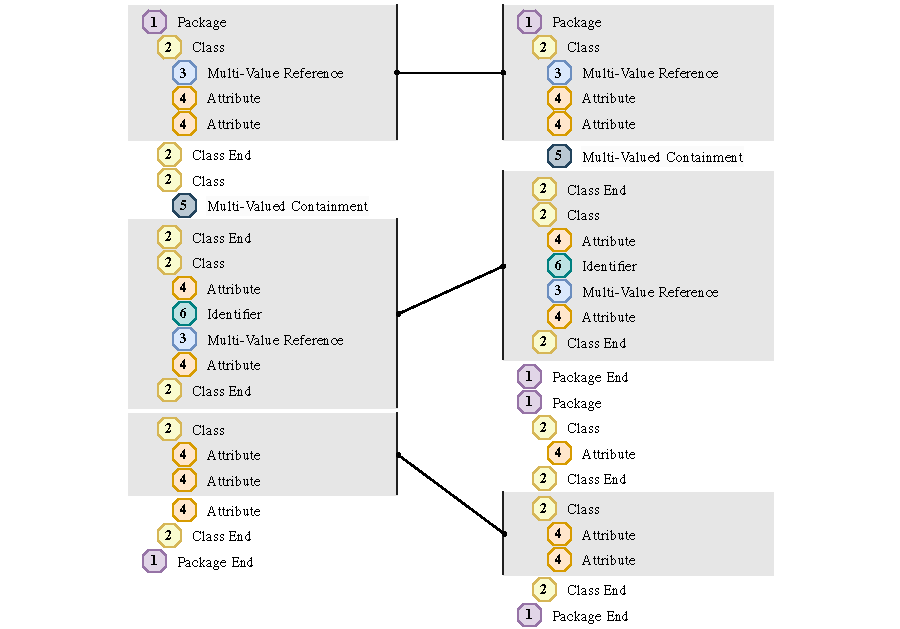
\includegraphics[width=\linewidth]{figures/mde/tokenMatching.pdf}
    \caption[Subsequence Matching for Modeling Artifacts]{Subsequence matches for the two token sequences of our running example in \autoref{fig:running-example} with a minimal token match of three. Three subsequences are matched with five, seven, and three tokens, respectively. The indentation solely serves illustrative purposes.}
    \label{fig:comparison}
\end{figure}

% ------------------------------------------------------------------
% 4. SIMILARITY CALCULATION
% ------------------------------------------------------------------

\section{Similarity Calculation}\label{subsec:similarity}

\noindent
The similarity calculation step remains unchanged when adapting token-based methods for detecting plagiarism in modeling assignments. Thus, we only briefly discuss this step.
As discussed in \autoref{sec:threatmodel-algebra}, the similarity of each modeling assignment pair can be calculated based on the subsequence matches.
For an assignment pair, the similarity can be calculated based on their token sequences with the symmetric similarity (\autoref{theo:avgsim}) or maximum similarity (\autoref{theo:maxsim}) metrics.
For pairs of assignments of different sizes, the maximum similarity can be used.
For pairs of assignments of different sizes, the maximum similarity is less resilient against false positives but better suited if many elements were inserted to obfuscate the plagiarism. We then use both metrics to rank pairs regarding their similarity. For our example in \autoref{fig:comparison}, the similarities are calculated to be $avgsim = 68.3\%$ and $maxsim = 71.4\%$, respectively.
%
Using these metrics, we can apply a wide variety of different post-processing to enhance the results for human inspection.
In practice, the following post-processing methods are commonly applied:
\begin{enumerate}[leftmargin=*]
    \item Ranked Lists of Pairs: A ranked list showing assignment pairs in descending order by similarity provides a prioritization for human inspection. Interactive refinements, such as filtering by similarity thresholds or excluding common template code, can streamline this process.
    \item Similarity Distribution: A histogram showing the distribution of similarity values for all comparisons, thus allowing us to identify what level of similarity is common for two given programs (probable true negatives) and what level of similarity indicates a comparison is an outlier (probable true positives).
    \item Clustering of Assignments: Using hierarchical agglomerative or spectral clustering to classify pairs according to their similarity helps detect group plagiarism.
    For the spectral clustering, automatic hyper-parameter search with Bayesian optimization using a Gaussian process as the surrogate model and L-BFGS for optimization \citet{Ng2001} can be employed. Configurable hyperparameters allow adaptation to different contexts, ensuring flexibility in analysis.
\end{enumerate}

These similarity metrics and post-processing techniques provide a robust foundation for educators to analyze the results of the plagiarism detection process. We ensure that individual and group plagiarism can be effectively identified via clustering analysis. This layered approach enhances detection quality and streamlines the subsequent human inspection process, making it more efficient in real-world educational settings.

% ------------------------------------------------------------------
% 5. VIZUALISATION
% ------------------------------------------------------------------

\section{Visualization}\label{subsec:visualization}


\noindent
An essential benefit of token-based approaches is the explainability of the calculated similarities. Moss~\cite{MOSS} and JPlag~\cite{prechelt2000}, for example, offer inspection of pairs of programs in a side-by-side code view, where the matched sections are highlighted. This facilitates the human assessment of the results and effective decision-making regarding what constitutes plagiarism. Providing this feature is crucial for the practical usage of plagiarism detectors \cite{Le2013}.
%
Graphical syntax and custom editors are commonly used to view and edit modeling artifacts. However, textual syntaxes benefit from linear structures that allow visualizing matches in a manner educators are used to from code plagiarism detectors. Nevertheless, a linear graphical syntax like a tree view also brings these benefits.

A suitable graphical or textual syntax has to be chosen for each modeling language. This makes this visualization step inherently domain-specific. This problem does not exist for code, as the persistent form of program code is the same form humans use to read and edit. For models, the persisted forms are rarely human-readable and do not reflect how they are viewed.

If a textual syntax is available, we propose using a side-by-side view based on textual syntaxes, thus effectively linearizing the modeling artifact.
The choice of textual syntax has to be domain-specific. For example, for \ac{EMF} metamodels, \textit{Emfatic}~\cite{Emfatic} allows us to depict them in a side-by-side view.
If no suitable textual syntax is available for a domain, a rudimentary solution is to implement a simple tree-based view based on the model elements and their tokenization references.

\begin{figure}
    \centering
    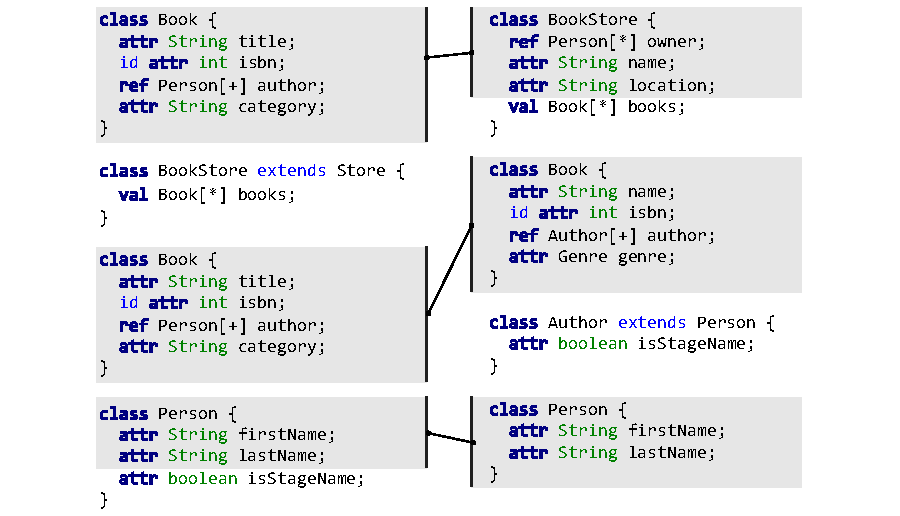
\includegraphics[width=\linewidth]{figures/mde/comparisonView.pdf}
    \caption[Visualization of Detected Modeling Plagiarism]{Textual representation of the matched metamodels fragments of our running example in \autoref{fig:running-example} via the Emfatic textual syntax~\cite{Emfatic}. This representation is similar to the typical visualization in source code plagiarism detection.}
    \label{fig:visualization}
\end{figure}

\autoref{fig:visualization} illustrates such a match visualization for the running example, which we calculated to be a 68.3 percent match. Emfatic is used to visualize the similarities between the metamodels. The three matches of \autoref{fig:comparison} are now traced back to the actual model elements. We observe that the class \texttt{Store} on the left side matches the class \texttt{BookStore} on the right side.
We also observe that the reference \texttt{books} on the right side is not matched, as it is part of the superclass \texttt{BookStore} on the left side. Furthermore, the classes called \texttt{Book} on both sides match despite different names and types of structural features. Finally, while both classes called \texttt{Person} match, the \texttt{isStageName} attribute is again moved into a superclass on the right side.
During human inspection, it is comprehensible how the similarity scores were calculated, and which parts are similar.
Even for such small models as depicted in \autoref{fig:running-example}, the side-by-side view in \autoref{fig:visualization} eases the comparison.


\section{Limitations}\label{sec:mde-limits}
In the following, we present two limitations of our approach.
First, we discuss the solution space problem, which is inherent to any plagiarism detection approach.
Second, we discuss the impact of the modeling domain and language on the effectiveness of our approach.

\subsection*{Domain-specific Tokenization}
As previously discussed, a generic tokenization strategy, which applies to a given model, will usually perform significantly worse for most models than a domain-specific one. Consequently, this makes finding a suitable mapping from model elements to tokens an inherently domain-specific problem. Thus, we cannot provide a universal solution for any given modeling domain or language. As an analogy, finding such a solution is like creating a universal model transformation that transforms between instances of any given metamodel. Any proposed solution would either be so broad that it lacks any purpose or would just not be universal.
While we provided a general framework and outlined the tokenization for the tokenization of \ac{EMF} models, it is up to the domain expert to find a suitable solution for a given modeling domain.
This limitation, however, is not unique to modeling languages, as existing literature does not provide detailed guidance for the tokenization of new programming language~\cite{Maertens2022, prechelt2002, prechelt2000, Joy1999}. Instead, examples are given for an exemplary programming language.

\subsection*{Wider Impact of the Modeling Domains}\label{sec:mde-limit-domain}
The effectiveness of our token-based plagiarism detection approach may vary depending on the modeling domain and language. It generally performs well for structural models and models where the semantic relationships form tree-based structures (e.g., containment trees). This covers most models used in \ac{MDE} education.
In some domains, however, models may represent highly abstract concepts with minimal structural detail, limiting the granularity available for tokenization. When structure is sparse or abstract, it becomes challenging to capture distinctive features that would reliably differentiate one model from another. This factor may especially play a role in behavioral models.

Further, the strength of semantic relationships (see \autoref{subsec:tokenization}), which our approach relies on to identify the semantic structure of the model, can vary greatly between domains. Some domains have well-defined, unambiguous semantic relationships that can be tokenized effectively, while for others, it is difficult to derive a consistent tokenization strategy. An example of such a case is \ac{UML} use case models. Here, it is nontrivial to find an order in which to linearize the models. Even though these models contain both relationships and associations, more empirical evidence is required to assess if, for example, actors should be considered before subsystems regarding the linearization order.

In sum, while our approach can be adapted to various modeling domains, the modeling domain's inherent characteristics affect how well our method performs. This limitation underlines the importance of customizing tokenization strategies to specific domains.

\subsection*{The Solutions Space Problem}
As discussed in \autoref{sec:mde-challenges}, detecting plagiarism in small modeling assignments can be challenging since these models require unique characteristics to distinguish them from others. Even minor structure, syntax, or modeling similarities can result in false positives. Furthermore, small modeling tasks often rely on commonly used patterns, making it difficult to differentiate between plagiarism and coincidental similarities, as the solution space of these assignments is minimal.
However, this limitation is inherent to plagiarism detection and thus also applies to code and natural language (see \autoref{sec:SPD-problem}). Consequently, whether manual checks or an automated approach like a plagiarism detector are employed, if the assignment size or complexity falls below a certain threshold, the space of all possible solutions collapses, and it is no longer possible to distinguish plagiarism cases from random similarities between unrelated solutions. This thus applies to our approach as it does to any other. However, this may occur more frequently in modeling assignments due to the challenge of abstraction Level and granularity (see \autoref{sec:mde-challenges}).